\chapter{Methodology}
\label{sec:meth}

In order to generate and analyze cyber alert data it is important to understand the structure of generic NIDS alerts. The categorical features contained by each alert provide contextual information such as the what, where, and how an attack occurs. By understanding the structure and meaning of each alert feature it is possible to begin selecting which features are worth pursuing synthetic generation of. Furthermore, the selection of these features drives the structure of the generative model used. This section will detail three neural network architectures driven by the features selected from NIDS alerts. 

\section{Alert Structure and Feature Selection}

NIDS alerts are formed through the compilation of packet traffic seen by each machine on the network. These alerts use fixed rulesets and information collected from multiple packets to summarize the believed intent of network traffic. Features such as HTTP Request Information, Alert Category and Signature, Destination IP, Source IP, and more are all captured by alerts. A subset of alert features are shown in Fig. \ref{fig:alert}. 

It is important to note that not all features are populated in every alert and that most features are comprised of discrete categorical values. Additionally, many features are grouped into families of information. One example of this is the HTTP family, which includes Hostname, Method, Redirect, URL, and more.

\begin{figure}
	\centering
	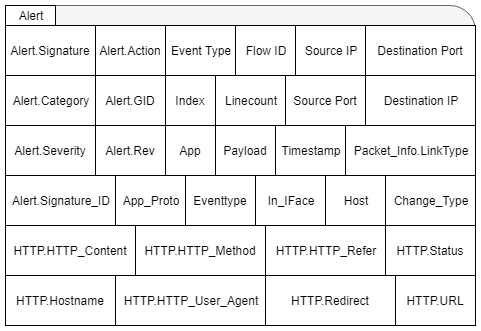
\includegraphics[width=.8\textwidth]{alert_struct}
	\caption{Sample NIDS Alert}
	\label{fig:alert}
\end{figure}

Given the wide variety of alert features available it is important to establish which alerts provide useful contextual information for future network alert modeling. Additionally, some of the features listed are generated through a fixed mapping from other features. For example, Alert Category is determined by a many to one mapping of Alert Signatures. Therefore, by generating Alert Signature it is possible to determine the Alert Category. 

When selecting features of an alert to use for any model it is important to consider the contextual data provided by that features. Features such as Alert Signature, Category, Action, and Eventtype provide the what and how an attack is carried out over the network. Destination IP and Port and Source IP and Port provide where the attack originated from and where it's targeting.  And Timestamp provides not only when an attack occurs but also it's temporal location with respect to other alerts.


\section{GAN Models}
\label{sec:model_arch}
Two GAN implementations were created to generate artificial cyber alert data; a standard Wasserstein GAN with Gradient Penalty and an extension of this model which used a neural estimate of mutual information to regularize the generator output.  

\subsection{Wasserstein GAN with Gradient Penalty}
\label{sec:gan}
The Wasserstein GAN with Gradient Penalty makes no architectural changes to model structure compared to standard GANs. Rather, the loss function is modified to use the Earthmover Distance. This modification has been shown to create empirically better results and allows for flexibility in model selection adapted to the challenge at hand.

Since the goal of this work was to create individual NIDS alerts without temporal correlation a feed-forward network architecture was selected for both the generator and discriminator. Four alert features were selected for alert generation: Alert Signature, Destination Port, Timestamp, and Source IP. Despite this, the models employed could easily be scaled to consider n-many features. 

The generator consisted of 2 layers. The first layer sampled from noise space $\mathbb{Z}$ to a hidden representation. The next layer was directly responsible for each feature's output value. Since each of the four selected features was categorical one hot encoded representations were used to represent each unique value. This layer consisted of four individual mappings from the hidden representation to an output layer with cardinality equal to the number of unique values per feature. Finally, a concatenation was used to take the prior 4 outputs and create a full 1-hot encoded alert. 

The discriminator also consisted of 2 layers. The first layer took 1-hot encoded alerts as input and mapped them to a hidden representation. The next layer mapped this hidden representation to a scalar value representing the probability that the alert was from the ground truth dataset. A graphical model is included in Fig. \ref{fig:model_simple}. Inputs to the network are highlighted in yellow. Learnable weight layers are in blue. The concatenation in orange is a non-backpropable layer used only to prepare generator output for input to the discriminator. The red boxes and lines represent the model loss functions and back-propagation.

\begin{figure}[!htbp]
	\centering%
	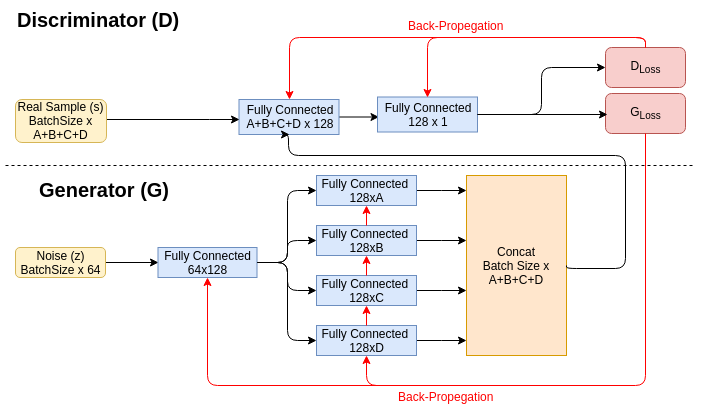
\includegraphics[width=\textwidth]{model_simple}
	\caption{WGAN-GP Model}
	\label{fig:model_simple}
\end{figure}

Table \ref{tab:model_simple_a} and Table \ref{tab:model_simple_b}, shows the dimensions of the weight matrices and activation functions for each layer of the network.

\begin{table}[!htbp]
	\centering
	\caption{Generator Network Architecture: Note that a-d are variable depending on the number of unique outputs}
	\label{tab:model_simple_a}
	\begin{tabular}{l|l|l}
		\hline
		\multicolumn{3}{c}{\textbf{Generator}} \\ 
		\hline
		\multicolumn{1}{c|}{Layer} & \multicolumn{1}{c|}{Matrix Dimensions} & \multicolumn{1}{c}{Activation Function} \\ \hline
		Input & 64 x 128 & ReLu \\
		Output - Feature 0 & 128 x A & NA \\
		Output - Feature 1 & 128 x B & NA \\
		Output - Feature 2 & 128 x C & NA \\
		Output  - Feature 3 & 128 x D & NA \\
		Concatenation & A+B+C+D & NA \\
		\hline
	\end{tabular}
\end{table}

\begin{table}[!htbp]
	\centering
	\caption{Discriminator Network Architecture: Note that a-d are variable depending on the number of unique outputs}
	\label{tab:model_simple_b}
	\begin{tabular}{l|l|l}
		\hline
		\multicolumn{3}{c}{\textbf{Discriminator}} \\ 
		\hline
		\multicolumn{1}{c|}{Layer} & \multicolumn{1}{c|}{Matrix Dimensions} & \multicolumn{1}{c}{Activation Function} \\ \hline
		Input & A+B+C+D x 128 & ReLu \\
		Output & 128 x 1 & Sigmoid \\
		\hline
	\end{tabular}
\end{table}


\subsection{Mutual Information Neural Estimator}
\label{sec:mine}
Mutual Information is a measure of dependence between two random variables. Traditionally, approximations have to be used to estimate the mutual information between high dimensional and continuous variables as exact computation is intractable. The Mutual Information Neural Estimator is a neural network which allows for state of the art approximation of mutual information. This is done by optimizing the network to minimize the Donsker-Varadhan representation of the KL divergence between two variables. 

A feed forward neural network was implemented to learn the mutual information between the gaussian noise sampled from $\mathbb{Z}$ and the generators output. This network consisted of 2 layers. The first layer took input from each of the aforementioned sources and mapped them to separate hidden representation layers and added together. Then the second layer mapped the hidden representation to a single output value representing the mutual information estimate. Table \ref{tab:model_mi} shows the matrix dimension for each of the layers in the network.

\begin{table}[!htbp]
	\centering
	\caption{Mutual Information Estimator Network Architecture: Note that a-d are variable depending on the number of unique outputs}
	\label{tab:model_mi}
	\begin{tabular}{l|l|l}
		\hline
		\multicolumn{3}{c}{\textbf{Estimator}} \\ 
		\hline
		\multicolumn{1}{c|}{Layer} & \multicolumn{1}{c|}{Matrix Dimensions} & \multicolumn{1}{c}{Activation Function} \\ \hline
		Input - Generated & A+B+C+D x 128 & NA \\
		Input - Noise & 64 x 128 & NA \\
		Addition & 128 & NA \\ 
		Output & 128 x 1 &  NA \\
		\hline
	\end{tabular}
\end{table}


\subsection{WGAN-GP with Mutual Information Constraint}
\label{sec:gpmi}

In order to improve mode dropping in the GAN model described in Section \ref{sec:gan} the mutual information neural estimator in Section \ref{sec:mine} is added to the model. This is done by using the mutual information between the generated samples and the input noise as a proxy for the neg-entropy of the samples. This regularizes the generator's weights and encourages full exploration of the feature space. We refer to this model as the Wasserstein GAN with Gradient Penalty and Mutual Information (WGAN-GPMI). Fig. \ref{fig:model_complex} shows what the full model consists of. The addition of the Mutual Information Estimation Network helps to enforce that the generator must learn all output modes of the distribution by fully exploiting the noise sample.

\begin{figure}[!htbp]
	\centering%
	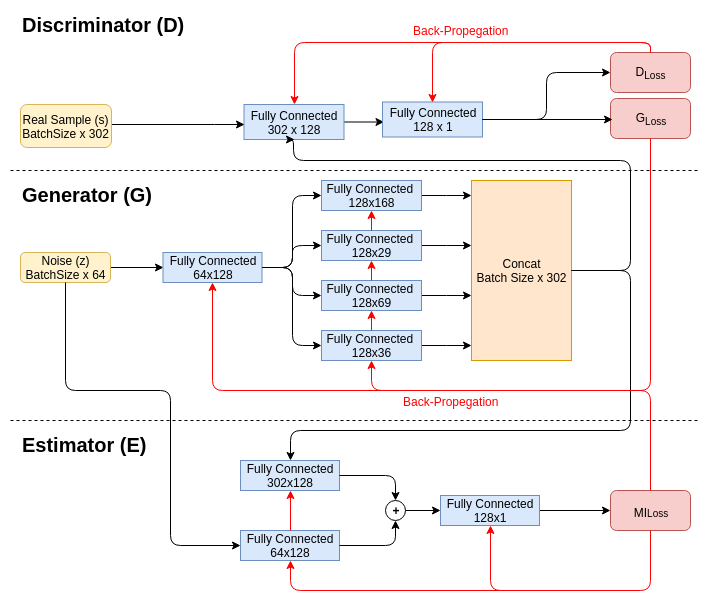
\includegraphics[width=\textwidth]{model_complex}
	\caption{WGAN-GPMI Model}
	\label{fig:model_complex}
\end{figure}

Since mutual information is theoretically unbounded, gradient updates resulting from it could overwhelm the adversarial gradients resulting from the Earthmover Distance. In order to address this all of the gradient updates to the generator are adaptively clipped to ensure that the Frobenius norm of the gradient resulting from the mutual information is at most equal to the adversarial gradient \cite{Belghazi2018}, as shown in (\ref{eq:fnorm}).

\begin{equation}
	g_{norm} = g_a + min(||{g_a}||, ||{g_m}||)({g_m \over ||g_m||})
	\label{eq:fnorm}
\end{equation}
 
Note that $g_{norm}$ is the normalized gradient, $g_a$ is the adversarial gradient resulting from (\ref{eq:WGAN-GP3}), and $g_m$ is the gradient resulting from (\ref{eq:MINE}). 

%\subsection{Model Training}
%\label{sec:training}

%Training GANs is a notoriously tricky task as loss score is not a fair representation of whether the model has converged to generating realistic data. Like many traditional Deep Learning models, hyperparameter tuning is critical to model performance for GANs. This creates a challenge while training GANs, especially with unconventional datasets where metrics like Inception Score cannot be applied. In order to address this and exhaustive hyperparameter search for each of the GAN models above was carried out. First, individual parameters were tuned in order to find candidate values. Then, these candidate values were used in a search of all possible parameter combinations.

%Using the histogram intersection metric proposed in Section \ref{sec:anal} across all combinations of features, the hyperparameter setting which achieved the most intersection scores in the $90^{th}$ percentile were selected as optimal. More details about the result of this search will be covered in Section \ref{sec:rna}.